\chapter{Introduction}
\textit{In this chapter, I provide the motivation for this project and setup the problem I am solving. I also explain some key algorithms involved. Finally, I cover some related work.}

\section{Motivation}
	
 Transmission Control Protocol (TCP) is the protocol of choice in many data centres. However, it is very sensitive to losses (by design, as a mean for congestion control), which can degrade the performance within the data centres significantly \cite{zilberman2017has}. Various congestion control, avoidance and recovery mechanisms are thus of high importance in this field to minimise such loss rate. Still, not all TCP losses are born equal. For example, losses happening at the destination host's network interface card (NIC) are not an indication of congestion within the network. It is assumed that fast retransmission of such lost packets, from within the network, can increase the utilisation of the network.
 
 In-network computing is an emerging research area in systems and networking, where applications traditionally running on the host are offloaded to the network hardware (e.g. switch, NIC). Examples of applications offloaded in the past include network functions (DNS server \cite{dns}), distributed systems functions such as consensus (P4xos \cite{p4xos}), various caching (netCache \cite{netCache}, netChain \cite{netChain}) and even a game (Tic-Tac-Toe). Key-Value Store (KVS) is also among the popular type of in-network applications. 
 
 Therefore, it is particularly interesting, and indeed challenging, to see how network-accelerated KVS concepts can be applied to TCP fast retransmit mechanism in order to improve cross-datacentre performance.
 
\section{Project Aims}
Fast retransmit is an enhancement to TCP that reduces the time a sender waits before retransmitting a lost segment. A TCP sender normally uses a simple timer to recognize lost segments. If an acknowledgement is not received for a particular segment within a specified time (a function of the estimated round-trip delay time), the sender will assume the segment was lost in the network, and will retransmit the segment.

Duplicate acknowledgement (DUP ACK) is the basis for the fast retransmit mechanism. After receiving a packet (e.g. with sequence number 1), the receiver sends an acknowledgement by adding 1 to the sequence number (i.e. acknowledgement number 2). This indicates to the sender that the receiver received the packet number 1 and it expects packet number 2. Suppose that three subsequent packets are lost. The next packets the receiver sees are packet numbers 5 and 6. After receiving packet number 5, the receiver sends an acknowledgement, but still only for sequence number 2. When the receiver receives packet number 6, it sends yet another acknowledgement value of 2. DUP ACK occurs when the sender receives more than one acknowledgement with the same sequence number (2 in our example).

When a sender receives several DUP ACKs, it can be reasonably confident that the segment with the sequence number specified in the DUP ACK was dropped. A sender with fast retransmit will then retransmit this packet immediately without waiting for its timeout.

\begin{figure}[h]
	\centering
	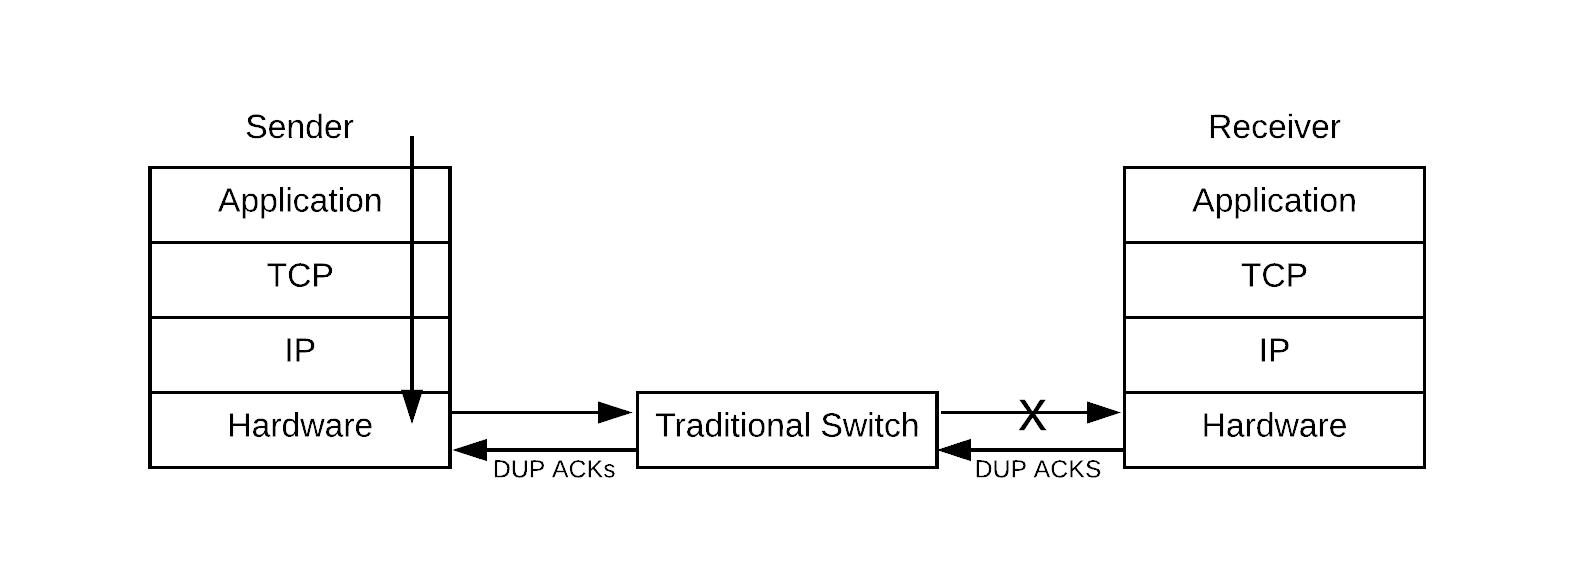
\includegraphics[width=\textwidth]{tradition-tcp.png}
	\caption{The standard convention of TCP handling.}
	\label{tradition-tcp}
\end{figure}

Currently, the DUP ACKs will traverse all the way back to the sender (\textbf{Figure \ref{tradition-tcp}}). The sender receives the DUP ACKs, then retransmits the packet with the next higher sequence number. 

\begin{figure}[h]
	\centering
	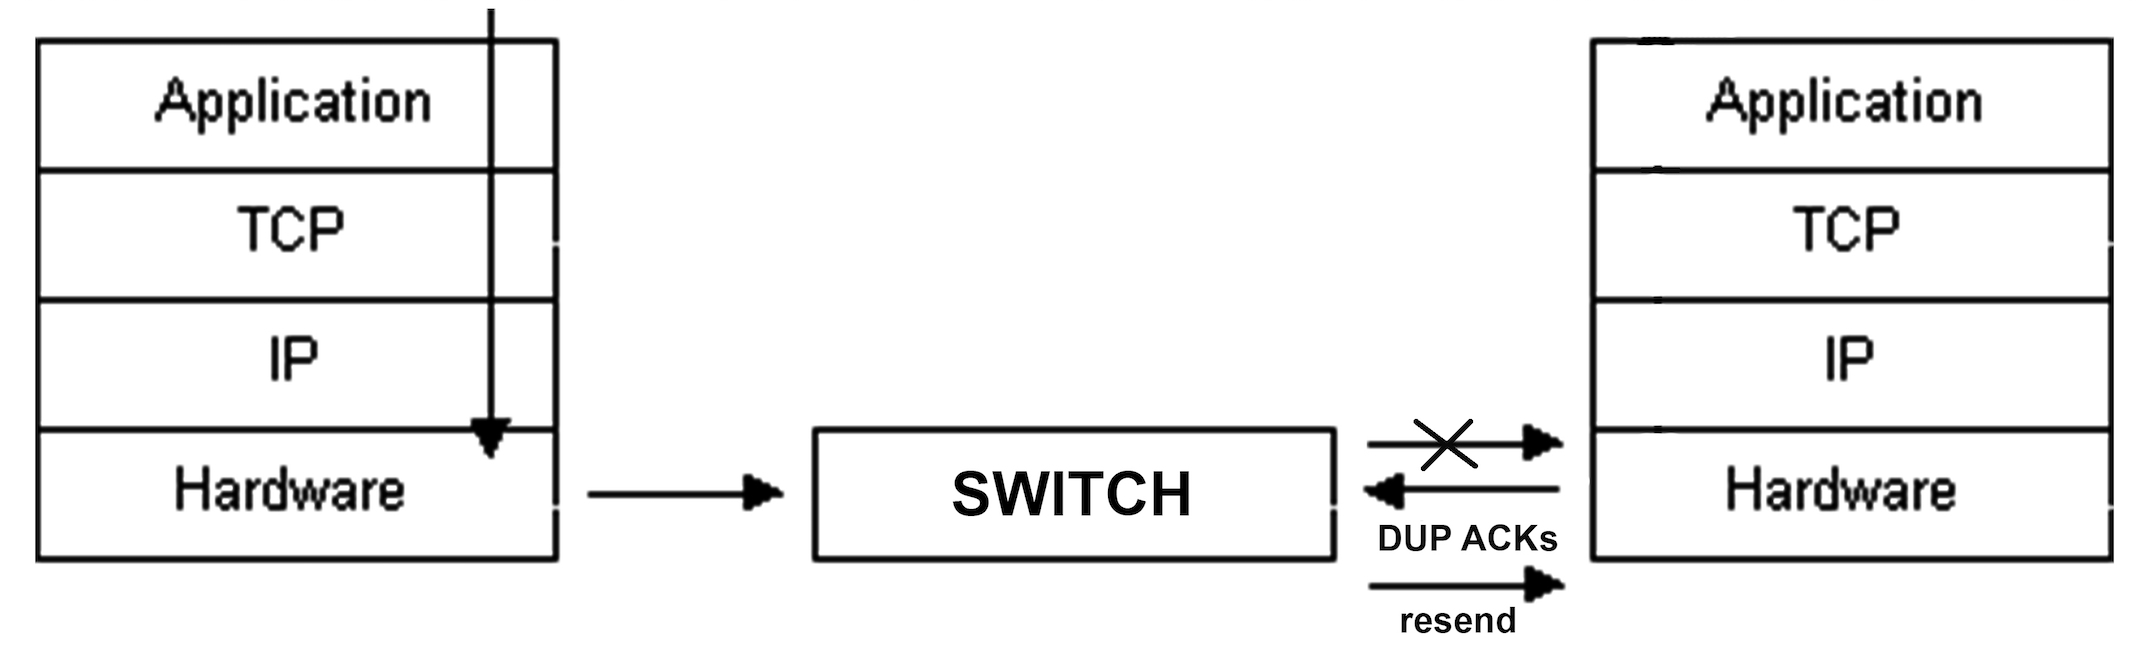
\includegraphics[width=\textwidth]{project-tcp.png}
	\caption{The proposed TCP handling.}
	\label{project-tcp}
\end{figure}

This project aims to design and implement a programmable switch that assists the TCP fast retransmit algorithm. The programmable switch will be able to retransmit the packets from within the network, instead of waiting for the DUP ACKs to get back to the host (\textbf{Figure \ref{project-tcp}}), thereby aims to reduce the response time to DUP ACKs and reduce unnecessary changes to the congestion window. The implementation will be based on the KVS concept, where the keys are the flow ID and the packet sequence number, and the value is the payload.

\section{Related Work}
	\subsection{TCP Congestion Control}
	One of the main aspects of TCP is congestion control, where a number of mechanisms are used to achieve high performance and avoid sending more data than the network is capable of forwarding, that is, to avoid causing network congestion. In particular, TCP uses a \textit{congestion avoidance} algorithm that includes various aspects of an additive increase/multiplicative decrease (AIMD) scheme, with other schemes such as \textit{slow start}, \textit{fast retransmit} and \textit{fast recovery} to achieve congestion avoidance. 
	
	The four intertwined algorithms are defined in more detail in RFC 5681\cite{rfc5681}. In this project, we are mostly interested in the \textit{fast retransmit} algorithm, which has been explained in the previous section.
	
	\subsection{Programmable Data Planes}
	In the last eight years, Software-defined Networking (SDN) and the OpenFlow protocol have reshaped the way people configure forwarding devices and determine network behaviour, by offering an open interface upon which apps like routing, monitoring, etc. can be built. OpenFlow has been the \textit{de facto} implementation of SDN. The key idea behind it was to decouple the control plane from the data plane, which allows centrally managing the control plane in software, while opening the control logic to the users. However, it is still very limited to a fixed set of features, which does not include new or custom protocols, statistics other than Packet, Byte count and Flow duration, and actions such as stateful matching or forwarding logic \cite{sdn}. This can change drastically with the re-emergence of programmable data planes and languages like P4 \cite{bosshart2014p4, p4spec, p4.org} and Protocol Oblivious Forwarding (POF) \cite{pof, song2013protocol}. They enable faster development/provisioning of new and/or custom protocols, as opposed to the long wait for the release of fixed-function Application-Specific Integrated Circuit (ASIC) switches supporting standardised protocols \cite{sivaraman2015dc}. Data plane programmability has the potential to unleash a new generation of future-proof forwarding devices, which are able to support major control plane and protocol updates, without mandating any hardware upgrades.

